\chapter{Teste da configuração do DNS} \label{Testing}

Para testar as configurações dos DNS, foi ativada a opção de logging no servidor DNS da rede de servidores para podermos analisar os pedidos DNS recebidos.
Os logs são escritos no ficheiro \verb|/var/log/query.log|.

\begin{figure}[H]
    \centering
    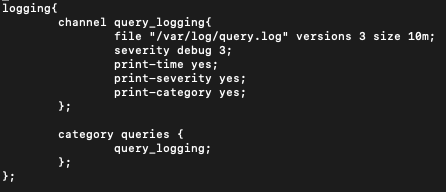
\includegraphics[width=.8\linewidth]{figs/logging/logging_conf.png}
    \caption{Configuração do Logging}
    \label{fig:logging_conf}
\end{figure}

É feito uso do comando \verb|dig| para fazer as queries DNS.
A razão para a utilização deste comando ao invés de \verb|nslookup| deve-se ao facto de ser possível discriminar a interface desejada.

\section{Split DNS} \label{split_dns}

O \textbf{Split DNS} vai separar os pedidos conforme o IP de origem.
Desse modo é de esperar:
\begin{itemize}
    \item Pedidos locais: Endereços da rede de servidores
    \item Pedidos Externos: Endereços da DMZ
\end{itemize}

\begin{figure}[H]
    \centering
    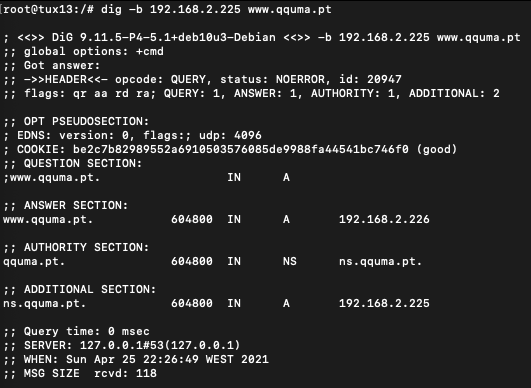
\includegraphics[width=.8\linewidth]{figs/logging/tux13_query_int.png}
    \caption{Query de um endereço local}
    \label{fig:tux13_query_int}
\end{figure}

\begin{figure}[H]
    \centering
    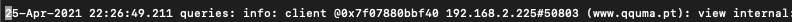
\includegraphics[width=.8\linewidth]{figs/logging/tux13_query_int_log.png}
    \caption{Log da query de endereço local}
    \label{fig:tux13_query_int_log}
\end{figure}

O endereço devolvido pela \textit{Query} é \verb|192.168.2.226|, que corresponde ao Webserver da rede de servidores.
No log é possível verificar que a \textit{view} do pedido é a interna, confirmado que reconhece o endereço local.


\begin{figure}[H]
    \centering
    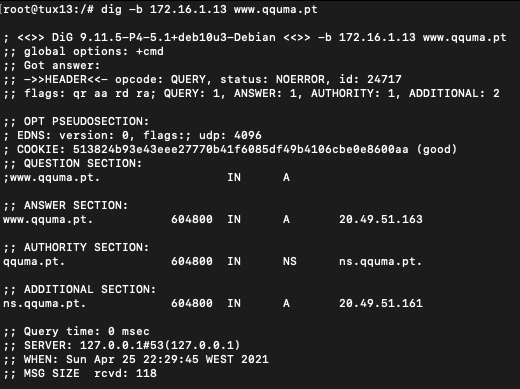
\includegraphics[width=.8\linewidth]{figs/logging/tux13_query_ext.png}
    \caption{Query de um endereço da DMZ}
    \label{fig:tux13_query_ext}
\end{figure}

\begin{figure}[H]
    \centering
    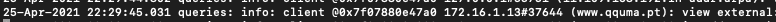
\includegraphics[width=.8\linewidth]{figs/logging/tux13_query_ext_log.png}
    \caption{Log da query de endereço da DMZ}
    \label{fig:tux13_query_ext_log}
\end{figure}

Neste caso, o endereço devolvido pela \textit{Query} é \verb|20.49.51.163|, que corresponde ao Webserver da DMZ.
Analogamente, no log é possível verificar que a \textit{view} do pedido é a externa, confirmado que filtra o pedido como externo.

É de notar que os pedidos tem um \textit{query time} de 0 ms, o que confirma que os pedidos são resolvidos localmente.

\clearpage 
\section{Loja} \label{loja_dns}

Os pedidos com origem na loja são tratados como pedidos locais pelo que devem ser devolvidos os endereços da rede de servidores, assim como o armazém.

\begin{figure}[H]
    \centering
    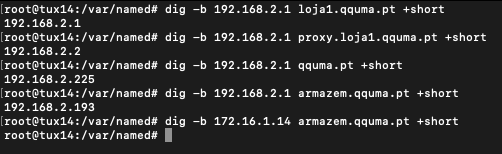
\includegraphics[width=.8\linewidth]{figs/logging/tux14_query.png}
    \caption{"Digs" na loja para endereços do sistema}
    \label{fig:tux14_query}
\end{figure}

Quando se faz dig para o endereço da loja, este devolve o próprio endereço da interface.
Apesar de o endereço da loja não estar definido no ficheiro \textit{database} do servidor DNS da rede de servidores,
o pedido é reencaminhado para o slave que é neste caso o servidor DNS da loja.
Este servidor tem na sua \textit{database} os \textit{DNS Records} dos domínios da loja, pelo que se confirma o correto funcionamento da tipologia \textit{Master-Slave}.

O \textit{Query} para o armazém é bem sucedido dado que o pedido é local. Externo não era possível resolver.

\section{Armazém} \label{arm_dns}

No caso do armazém, este não consegue resolver nenhum pedido, pelo que todos são reencaminhados para a rede de servidores.

\begin{figure}[H]
    \centering
    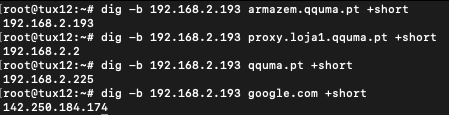
\includegraphics[width=.8\linewidth]{figs/logging/tux12_query.png}
    \caption{"Digs" no armazém para endereços do sistema}
    \label{fig:tux12_query}
\end{figure}

Como de esperar, todas as \textit{queries} são resolvidas corretamente como endereços locais, incluíndo a \textit{query} para o próprio armazém.
